\documentclass[12pt, titlepage]{article}
\pdfinfoomitdate=1
\pdftrailerid{}

\usepackage{booktabs}
\usepackage{tabularx}
\usepackage{hyperref}
\hypersetup{
    colorlinks,
    citecolor=blue,
    filecolor=black,
    linkcolor=red,
    urlcolor=blue
}
\usepackage[round]{natbib}
\usepackage{pifont}
\usepackage{booktabs,tabularx}
\usepackage{float}
\usepackage{array}
\usepackage{amssymb}
\usepackage{amsmath}
\usepackage{graphicx}
\usepackage{xcolor}
\usepackage{caption, subcaption}
\usepackage{enumitem}
\usepackage{multirow}
\usepackage{pgfplots}
\pgfplotsset{compat=1.18}
\usepgfplotslibrary{groupplots}
\usepackage{algorithm}
\usepackage{algpseudocode}

\input{../../Comments}
\input{../../Common}

\graphicspath{{report_figures/}{../../../assets/logo/}}

\begin{document}

\title{Robust Small Rocket Detection with YOLO26s:\\
Aggressive Augmentation Training and FP16 Edge Deployment}
\author{\authname}
\date{March 2026}

\maketitle

\begin{abstract}
  We present the training methodology and deployment pipeline for a
  small-rocket detection system designed for real-time edge inference on
  the NVIDIA Jetson Orin Nano.  Using \textsc{Yolo26s} (9.47M parameters,
  stride $\{8, 16, 32\}$), we train with aggressive data augmentation
  centred on \textbf{full mosaic} ($\text{mosaic}=1.0$), multi-scale
  input ($544$--$960$\,px), and 7~custom Albumentations transforms
  targeting real-world imaging degradation.  The model is trained for 420
  epochs on 15{,}832 rocket images supplemented with 4{,}000 COCO hard
  negatives, achieving validation
  $\text{mAP}_{50\text{-}95} = 0.694$ and $\text{mAP}_{50} = 0.947$.
  After ONNX export and TensorRT FP16 compilation, the deployed model
  achieves \textbf{DeepStream $\text{mAP}_{50\text{-}95} = 0.631$},
  $\text{mAP}_{50} = 0.875$, and
  $\text{mAP}_{50\text{-}95}(\text{small}) = 0.341$ on the Jetson Orin
  Nano.  We additionally investigate the \textsc{Yolo26s-P2} variant
  (stride-4 detection head), which achieves superior training metrics
  ($\text{mAP}_{50\text{-}95} = 0.765$) but suffers catastrophic
  degradation under FP16 quantisation ($0.765 \to 0.539$), confirming
  that \textbf{deployment-validated accuracy} must guide model selection
  over training-only metrics.  All experiments are conducted on NVIDIA
  H100 GPUs at McMaster University's Grace HPC cluster.
\end{abstract}

\pagenumbering{roman}

\section*{Revision History}

\begin{tabularx}{\textwidth}{p{3cm}p{2cm}X}
  \toprule {\bf Date} & {\bf Version} & {\bf Notes}                                \\
  \midrule
  2026-03-01          & 1.0           & Initial draft (V1 pipeline)                \\
  2026-03-03          & 2.0           & Added V1 experimental results              \\
  2026-03-10          & 2.1           & Renamed from CVReport to MLReport          \\
  2026-03-26          & 3.0           & Added V2/V3 P2 pipeline (not deployed)     \\
  2026-03-28          & 4.0           & Major rewrite: refocused on deployed
  smallrocket model (train63), added deployment pipeline and FP16
  benchmark results, documented P2 failure as lesson learned            \\
  \bottomrule
\end{tabularx}

~\\

\newpage

\tableofcontents

\newpage

\section{Symbols, Abbreviations, and Acronyms}

\renewcommand{\arraystretch}{1.2}
\begin{tabular}{l l}
  \toprule
  \textbf{Symbol}      & \textbf{Description}                                                \\
  \midrule
  mAP                  & Mean Average Precision --- object detection evaluation metric       \\
  mAP$_{50}$           & mAP at IoU threshold 0.50                                           \\
  mAP$_{50\text{-}95}$ & mAP averaged across IoU thresholds 0.50 to 0.95                     \\
  DS mAP               & mAP measured on DeepStream FP16 deployment                          \\
  YOLO                 & You Only Look Once --- real-time object detection architecture      \\
  COCO                 & Common Objects in Context --- large-scale object detection dataset  \\
  SGD                  & Stochastic Gradient Descent --- optimisation algorithm              \\
  GFLOPs               & Giga Floating Point Operations --- computational complexity measure \\
  P2 head              & Stride-4 detection head in YOLO architecture                        \\
  AMP                  & Automatic Mixed Precision --- FP16/FP32 hybrid training             \\
  TensorRT             & NVIDIA inference optimisation SDK with FP16/INT8 quantisation       \\
  DeepStream           & NVIDIA SDK for GPU-accelerated video analytics pipelines            \\
  ONNX                 & Open Neural Network Exchange --- model interchange format           \\
  \bottomrule
\end{tabular}\\

\newpage

\pagenumbering{arabic}

%% ====================================================================
\section{Introduction}
\label{sec:intro}
%% ====================================================================

Detecting small, fast-moving rockets in surveillance footage poses unique
challenges for modern object detectors.  The targets of interest typically
occupy fewer than $30{\times}30$ pixels in $960{\times}960$ frames, can appear
at \emph{any} orientation ($0$--$360^{\circ}$), and are subject to imaging
degradation including motion blur, compression artefacts, and varying
illumination.

The \progname{} system requires \textbf{real-time inference on edge hardware}
--- specifically the NVIDIA Jetson Orin Nano (8\,GB), running a DeepStream
pipeline with TensorRT FP16 quantisation.  This deployment constraint
introduces a critical gap between training-time and deployment-time accuracy:
models that excel in FP32 validation may degrade significantly under FP16
quantisation, particularly architectures with high-resolution feature maps.

The YOLO family of detectors~\citep{ultralytics2025yolo} offers an attractive
balance between speed and accuracy for real-time deployment.  We select
\textsc{Yolo26s} (9.47M parameters, stride $\{8, 16, 32\}$) as our
architecture, trained with an aggressive augmentation strategy centred on
\textbf{full mosaic augmentation} ($\text{mosaic} = 1.0$) and multi-scale
training.

\noindent Our contributions include:

\begin{enumerate}[leftmargin=*]
  \item \textbf{Deployment-validated training}: end-to-end pipeline from
        training on H100 GPUs to FP16 benchmark on Jetson Orin Nano, with
        deployment metrics as the primary selection criterion.
  \item \textbf{Full mosaic augmentation}: demonstration that
        $\text{mosaic} = 1.0$ is critical for small-object detection, with
        all reduced-mosaic variants failing to match baseline performance.
  \item \textbf{COCO hard negative mining}: 4{,}000 background images
        ($\sim\!25\%$ of training set) to suppress false positives.
  \item \textbf{Multi-scale training}: variable input resolution
        ($544$--$960$\,px) for scale-invariant feature learning.
  \item \textbf{P2 failure analysis}: documentation that the stride-4
        detection head, despite $+10\%$ training mAP, suffers $-30\%$
        deployment degradation under FP16 quantisation.
\end{enumerate}

%% ====================================================================
\section{Dataset}
\label{sec:dataset}
%% ====================================================================

\subsection{ROCAM Dataset}

The ROCAM dataset is a single-class (\texttt{rocket}) object detection dataset
derived from surveillance camera footage of rocket launches.

\begin{table}[h]
  \centering
  \caption{ROCAM dataset statistics.}
  \label{tab:dataset}
  \begin{tabular}{@{}lrrr@{}}
    \toprule
    \textbf{Split}     & \textbf{Images}   & \textbf{Labels} & \textbf{Notes}             \\
    \midrule
    Train (original)   & 11{,}832          & 11{,}832        & Annotated rockets          \\
    Train (+ COCO neg) & 15{,}832          & 15{,}832        & +4{,}000 background images \\
    Validation         & 3{,}378           & 3{,}378         &                            \\
    \midrule
    \textbf{Total}     & \textbf{19{,}210} &                 & Single class               \\
    \bottomrule
  \end{tabular}
\end{table}

Annotations follow the YOLO format (class, $x_c$, $y_c$, $w$, $h$ normalised
to $[0,1]$).  Training uses rectangular multi-scale input with base resolution
$544 {\times} 960$.

\subsection{Target Size Distribution}
\label{sec:target_size}

A critical characteristic of this dataset is the extreme range of target
sizes.  Table~\ref{tab:size_dist} shows the distribution at
$\text{imgsz}=960$.

\begin{table}[h]
  \centering
  \caption{Target size distribution at $960{\times}960$ resolution.  Sizes
    are measured as $\max(w, h)$ in pixels.  Total bounding boxes: 12{,}976.}
  \label{tab:size_dist}
  \begin{tabular}{@{}lrr@{}}
    \toprule
    \textbf{Size Range}            & \textbf{Count} & \textbf{Proportion} \\
    \midrule
    $<10$\,px (very small)         & 214            & 1.6\%               \\
    $10$--$20$\,px                 & 454            & 3.5\%               \\
    $20$--$32$\,px                 & 622            & 4.8\%               \\
    $32$--$50$\,px                 & 997            & 7.7\%               \\
    $50$--$100$\,px                & 2{,}441        & 18.8\%              \\
    $100$--$200$\,px               & 3{,}014        & 23.2\%              \\
    $>200$\,px                     & 5{,}234        & 40.3\%              \\
    \midrule
    \textbf{COCO-small ($<32$\,px)} & \textbf{1{,}290} & \textbf{9.9\%}  \\
    \bottomrule
  \end{tabular}
\end{table}

Nearly 10\% of targets fall below the COCO-small threshold of 32\,px, making
small-object augmentation strategy a decisive factor in model performance.

\subsection{COCO Hard Negative Mining}
\label{sec:coco_neg}

To suppress false positives, we inject \textbf{4{,}000 pure background images}
from MS~COCO~\citep{lin2014coco} into the training set.  Images are randomly
sampled (seed$=0$) from COCO train2017 and val2017 (${\sim}123$K total), copied
into the training directory with empty label files to provide pure background
supervision.

\begin{algorithm}[h]
  \caption{COCO Hard Negative Mining Pipeline}
  \label{alg:coco}
  \begin{algorithmic}[1]
    \Require COCO train2017 + val2017 images (${\sim}123$K total)
    \Require Target count $N = 4{,}000$
    \State Download and extract COCO images (cached after first run)
    \State $S \gets \textsc{RandomSample}(\text{all COCO images}, N, \text{seed}=0)$
    \For{each image $s_i \in S$}
    \State Copy $s_i$ to \texttt{images/train/coco\_neg\_\{i\}.jpg}
    \State Create empty label file \texttt{labels/train/coco\_neg\_\{i\}.txt}
    \EndFor
  \end{algorithmic}
\end{algorithm}

The empty label files ensure YOLO treats these images as containing \emph{zero}
objects.  At 25.3\% of the training set, the COCO negatives force a harder
decision boundary, which is critical for suppressing false positives during
real-world deployment.

%% ====================================================================
\section{Model Architecture}
\label{sec:arch}
%% ====================================================================

\subsection{YOLO26s}

YOLO26~\citep{ultralytics2025yolo} is the latest generation of the Ultralytics
YOLO family, featuring an updated backbone and a dual-head design.  The
\textbf{small} variant (\textsc{Yolo26s}) provides an optimal balance between
accuracy and inference speed for edge deployment.

\begin{table}[h]
  \centering
  \caption{\textsc{Yolo26s} architecture summary.}
  \label{tab:arch}
  \begin{tabular}{@{}lc@{}}
    \toprule
    \textbf{Property}         & \textbf{Value}          \\
    \midrule
    Parameters                & 9.47M                   \\
    Layers                    & 454                     \\
    Detection strides         & $\{8, 16, 32\}$         \\
    Detection heads           & 3                       \\
    Pretrained weights        & COCO (yolo26s.pt)       \\
    \bottomrule
  \end{tabular}
\end{table}

The standard 3-head architecture with strides $\{8, 16, 32\}$ was selected over
the P2 variant (stride-4 head) based on deployment testing.  While the P2
variant achieves higher training metrics, it suffers catastrophic FP16
quantisation loss (Section~\ref{sec:p2_failure}).

%% ====================================================================
\section{Training Methodology}
\label{sec:method}
%% ====================================================================

\subsection{Training Configuration}

The model is trained from COCO-pretrained weights (\texttt{yolo26s.pt}) for
420 epochs on a single NVIDIA H100 GPU.  Table~\ref{tab:train_config} lists
the complete training configuration.

\begin{table}[H]
  \centering
  \caption{Complete training configuration (train63).}
  \label{tab:train_config}
  \begin{tabular}{@{}ll@{}}
    \toprule
    \textbf{Parameter}    & \textbf{Value}                                    \\
    \midrule
    Model                 & \texttt{yolo26s.pt} (COCO pretrained)             \\
    Image size            & $(544, 960)$ with multi-scale                     \\
    Batch size            & 64                                                \\
    Epochs                & 420                                               \\
    GPU                   & 1$\times$H100 PCIe (80\,GB)                       \\
    Precision             & Mixed (AMP, FP16/FP32)                            \\
    Cache                 & Disk                                              \\
    Workers               & 8                                                 \\
    \midrule
    Optimiser             & SGD (auto)                                        \\
    $\text{lr}_0$         & 0.01                                              \\
    $\text{lrf}$          & 0.01 (linear decay)                               \\
    $\cos\_\text{lr}$     & False                                             \\
    Momentum              & 0.937                                             \\
    Weight decay          & 0.0005                                            \\
    NBS                   & 64                                                \\
    Warmup epochs         & 3.0                                               \\
    Warmup bias lr        & 0.1                                               \\
    Warmup momentum       & 0.8                                               \\
    \midrule
    Patience              & 30                                                \\
    Save period           & 25                                                \\
    Seed                  & 0                                                 \\
    Deterministic         & False                                             \\
    \bottomrule
  \end{tabular}
\end{table}

\subsection{Multi-Scale Training}
\label{sec:multiscale}

Multi-scale training (\texttt{multi\_scale=True}) varies the input resolution
between $544$ and $960$ pixels during training.  This forces the model to
learn scale-invariant features, which is particularly important for our
dataset where target sizes span from $<10$\,px to $>200$\,px.  The base
resolution of $(544, 960)$ is a rectangular aspect ratio matching the
surveillance camera's native format.

\subsection{Loss Weights}

\begin{table}[h]
  \centering
  \caption{Loss function weights.}
  \label{tab:loss}
  \begin{tabular}{@{}lc@{}}
    \toprule
    \textbf{Loss Component}    & \textbf{Weight} \\
    \midrule
    Box loss                   & 7.5             \\
    Classification loss        & 0.5             \\
    Distribution focal loss    & 1.5             \\
    \bottomrule
  \end{tabular}
\end{table}

%% ====================================================================
\section{Data Augmentation Strategy}
\label{sec:augmentation}
%% ====================================================================

\subsection{The Critical Role of Full Mosaic}
\label{sec:mosaic}

The single most important augmentation decision is setting
$\texttt{mosaic} = 1.0$, meaning \textbf{every training image} is composed
as a $2{\times}2$ mosaic of four random images.  This produces three key
effects:

\begin{enumerate}[leftmargin=*]
  \item \textbf{Object density}: Each mosaic tile contains a full image
        scaled to $\frac{1}{4}$ area, quadrupling the effective object density
        per training sample.
  \item \textbf{Scale diversity}: The $\frac{1}{4}$-scale mosaic tiles
        create additional small-object examples, directly augmenting the
        under-represented COCO-small category.
  \item \textbf{Context mixing}: Objects appear against varied backgrounds
        from different images, improving generalisation.
\end{enumerate}

Mosaic is disabled for the final 80 epochs (\texttt{close\_mosaic=80}) to
allow the model to refine on full-resolution images.  This two-phase
approach is essential: full mosaic builds robust features, then full-resolution
training sharpens localisation.

\paragraph{Empirical validation.}  All experiments with reduced mosaic
($\text{mosaic} < 1.0$) failed to match the baseline's deployment performance.
Table~\ref{tab:mosaic_ablation} summarises the evidence.

\begin{table}[H]
  \centering
  \caption{Effect of mosaic probability on deployment mAP.  All reduced-mosaic
    variants underperform the $\text{mosaic}=1.0$ baseline.}
  \label{tab:mosaic_ablation}
  \small
  \begin{tabular}{@{}llcccc@{}}
    \toprule
    \textbf{Experiment} & \textbf{mosaic} & \textbf{close\_mosaic} &
    \textbf{Val mAP} & \textbf{DS mAP} & \textbf{DS small} \\
    \midrule
    train63 (baseline)  & \textbf{1.0}    & 80                     &
    0.694             & \textbf{0.631}  & \textbf{0.341}    \\
    Plan~C (from scratch) & 0.80         & 150                    &
    0.646             & 0.499           & 0.238             \\
    Plan~F (small-obj)  & 0.30            & 60                     &
    ---               & ---             & ---               \\
    Plan~G (clone63 FT) & 1.0             & 80                     &
    0.645             & 0.621           & 0.282             \\
    \bottomrule
  \end{tabular}
\end{table}

\subsection{Geometric Augmentations}

\begin{table}[h]
  \centering
  \caption{Geometric augmentation parameters.}
  \label{tab:geo_aug}
  \begin{tabular}{@{}lcc@{}}
    \toprule
    \textbf{Parameter}    & \textbf{Value}   & \textbf{Rationale}              \\
    \midrule
    degrees               & 180              & Rockets at any orientation      \\
    flipud                & 0.5              & Vertical symmetry               \\
    fliplr                & 0.5              & Horizontal symmetry             \\
    shear                 & 5.0              & Perspective variation           \\
    perspective           & 0.0002           & Mild perspective warp           \\
    translate             & 0.05             & Position shift                  \\
    scale                 & 0.3              & Scale variation                 \\
    erasing               & 0.4              & Random erasing (occlusion)      \\
    \bottomrule
  \end{tabular}
\end{table}

The $\texttt{degrees}=180$ setting is critical: rockets can appear at any
orientation in the surveillance footage, so the model must be fully
rotation-invariant.

\subsection{Colour and Composition Augmentations}

\begin{table}[h]
  \centering
  \caption{Colour and composition augmentation parameters.}
  \label{tab:colour_aug}
  \begin{tabular}{@{}lcl@{}}
    \toprule
    \textbf{Parameter} & \textbf{Value} & \textbf{Rationale}              \\
    \midrule
    hsv\_h             & 0.015          & Hue jitter                      \\
    hsv\_s             & 0.6            & Saturation jitter               \\
    hsv\_v             & 0.4            & Value (brightness) jitter       \\
    mixup              & 0.1            & Image blending                  \\
    cutmix             & 0.1            & Region-based mixing             \\
    copy\_paste        & 0.0            & Disabled (baseline)             \\
    \bottomrule
  \end{tabular}
\end{table}

\subsection{Custom Albumentations Pipeline}
\label{sec:albumentations}

Seven custom Albumentations transforms target real-world imaging degradation
encountered in surveillance footage:

\begin{table}[H]
  \centering
  \caption{Custom Albumentations transforms for imaging robustness.}
  \label{tab:albumentations}
  \small
  \begin{tabular}{@{}llcl@{}}
    \toprule
    \textbf{Transform}            & \textbf{Parameters}            & \textbf{$p$} & \textbf{Purpose}              \\
    \midrule
    MotionBlur                    & blur\_limit$=7$                & 0.15         & Camera/target motion           \\
    GaussianBlur                  & blur\_limit$=7$                & 0.10         & Defocus simulation             \\
    GaussNoise                    & var\_limit$=(10, 50)$          & 0.15         & Sensor noise                  \\
    ImageCompression              & quality$=[40, 95]$             & 0.20         & JPEG artefacts                \\
    RandomBrightnessContrast      & ---                            & 0.20         & Illumination variation        \\
    RandomGamma                   & ---                            & 0.10         & Exposure differences          \\
    CLAHE                         & clip\_limit$=3.0$              & 0.10         & Local contrast enhancement    \\
    \bottomrule
  \end{tabular}
\end{table}

These transforms are passed via Ultralytics' native \texttt{augmentations}
parameter, ensuring reliable application during training.

%% ====================================================================
\section{Deployment Pipeline}
\label{sec:deployment}
%% ====================================================================

The deployment pipeline bridges the gap between training on H100 GPUs and
inference on the Jetson Orin Nano edge device.

\subsection{Export and Compilation}

\begin{enumerate}[leftmargin=*]
  \item \textbf{ONNX export} (on Grace/H100): The trained \texttt{best.pt}
        weights are exported to ONNX format using Ultralytics' export API
        with \texttt{simplify=True}.  This must be performed on the Grace
        server due to numpy PCG64 random state compatibility between
        numpy~2.x (Grace) and numpy~1.x (Orin).
  \item \textbf{Transfer}: The ONNX model is transferred to the Orin via
        \texttt{scp}.
  \item \textbf{TensorRT compilation} (on Orin): The ONNX model is compiled
        to a TensorRT engine with \textbf{FP16 precision} at the target
        deployment resolution.
\end{enumerate}

\subsection{DeepStream Integration}

The compiled TensorRT engine is integrated into NVIDIA DeepStream, which
provides a GPU-accelerated video analytics pipeline.  Accuracy is benchmarked
using a custom \texttt{accuracy\_benchmark.py} script that evaluates the
DeepStream pipeline's output against ground-truth annotations from the
validation set.

\subsection{FP16 Quantisation Considerations}

TensorRT FP16 quantisation reduces model weights and activations from FP32
to FP16, halving memory bandwidth and enabling Tensor Core acceleration.
However, FP16's reduced dynamic range (5-bit exponent vs.\ 8-bit in FP32)
can cause accuracy degradation, particularly in:

\begin{itemize}[leftmargin=*]
  \item High-resolution feature maps where small activation differences
        encode spatial precision.
  \item Architectures with many layers operating at fine spatial resolution
        (e.g., stride-4 heads).
\end{itemize}

\noindent The standard \textsc{Yolo26s} (minimum stride$=8$) is robust to
FP16 quantisation, with a manageable $0.694 \to 0.631$ accuracy gap
($-9.1\%$).  The P2 variant (minimum stride$=4$) is not
(Section~\ref{sec:p2_failure}).

%% ====================================================================
\section{Experimental Results}
\label{sec:results}
%% ====================================================================

\subsection{Training Metrics}

The model completes all 420 epochs without early stopping.

\begin{table}[H]
  \centering
  \caption{Final training validation metrics (epoch 419).}
  \label{tab:train_results}
  \begin{tabular}{@{}lc@{}}
    \toprule
    \textbf{Metric}             & \textbf{Value}       \\
    \midrule
    Precision                   & 0.945                \\
    Recall                      & 0.897                \\
    mAP$_{50}$                  & 0.947                \\
    mAP$_{50\text{-}95}$        & \textbf{0.694}       \\
    \bottomrule
  \end{tabular}
\end{table}

\subsection{Deployment Metrics (DeepStream FP16)}
\label{sec:deploy_results}

\begin{table}[H]
  \centering
  \caption{DeepStream FP16 benchmark results on Jetson Orin Nano.}
  \label{tab:deploy_results}
  \begin{tabular}{@{}lc@{}}
    \toprule
    \textbf{Metric}                      & \textbf{Value}       \\
    \midrule
    DS mAP$_{50}$                        & 0.875                \\
    DS mAP$_{50\text{-}95}$              & \textbf{0.631}       \\
    DS mAP$_{50\text{-}95}$ (small)      & \textbf{0.341}       \\
    \midrule
    Quantisation gap (mAP$_{50\text{-}95}$) & $-0.063$ ($-9.1\%$)\\
    \bottomrule
  \end{tabular}
\end{table}

The $-9.1\%$ quantisation gap is within acceptable range for FP16 deployment
and represents the production baseline that all improvement efforts must exceed.

\subsection{Training--Deployment Gap Analysis}

\begin{table}[H]
  \centering
  \caption{Training vs.\ deployment metric comparison.}
  \label{tab:gap}
  \begin{tabular}{@{}lccc@{}}
    \toprule
    \textbf{Metric}          & \textbf{Training (FP32)} & \textbf{DeepStream (FP16)} & \textbf{Gap}    \\
    \midrule
    mAP$_{50}$               & 0.947                    & 0.875                      & $-7.6\%$        \\
    mAP$_{50\text{-}95}$     & 0.694                    & 0.631                      & $-9.1\%$        \\
    \bottomrule
  \end{tabular}
\end{table}

\subsection{Training Curves}

\begin{figure}[H]
  \centering
  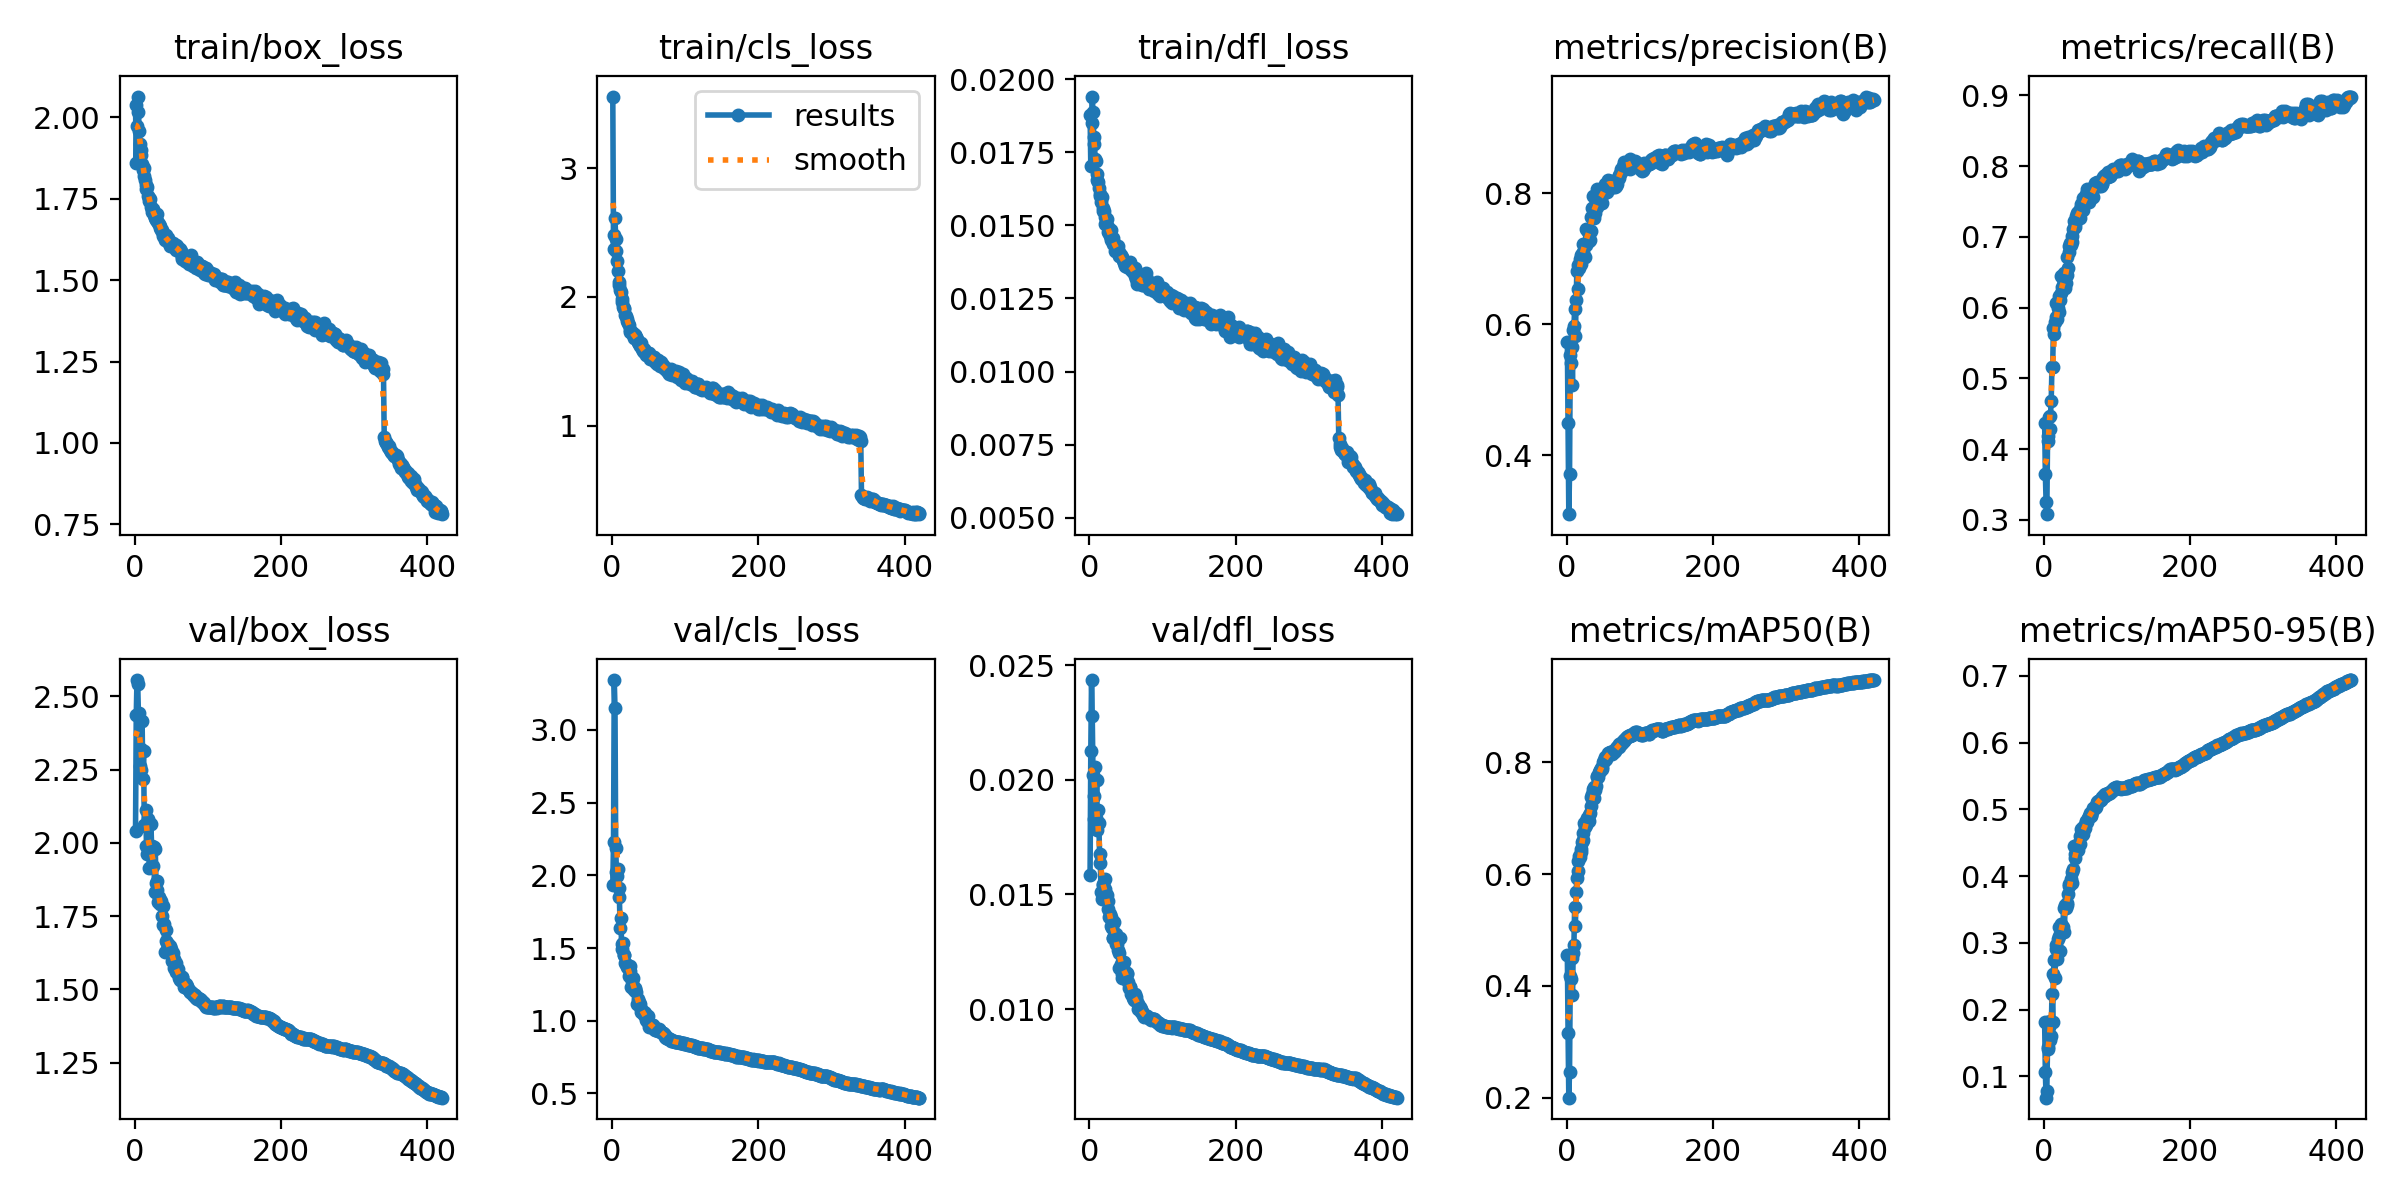
\includegraphics[width=0.7\textwidth]{results_train63.png}
  \caption{Training curves for the deployed model (train63, 420 epochs).
    The loss curves show steady convergence with a notable inflection after
    epoch~340 when mosaic augmentation is disabled
    (\texttt{close\_mosaic}$=80$).}
  \label{fig:train_curves}
\end{figure}

\subsection{Precision--Recall Analysis}

\begin{figure}[H]
  \centering
  \begin{subfigure}[t]{0.48\textwidth}
    \centering
    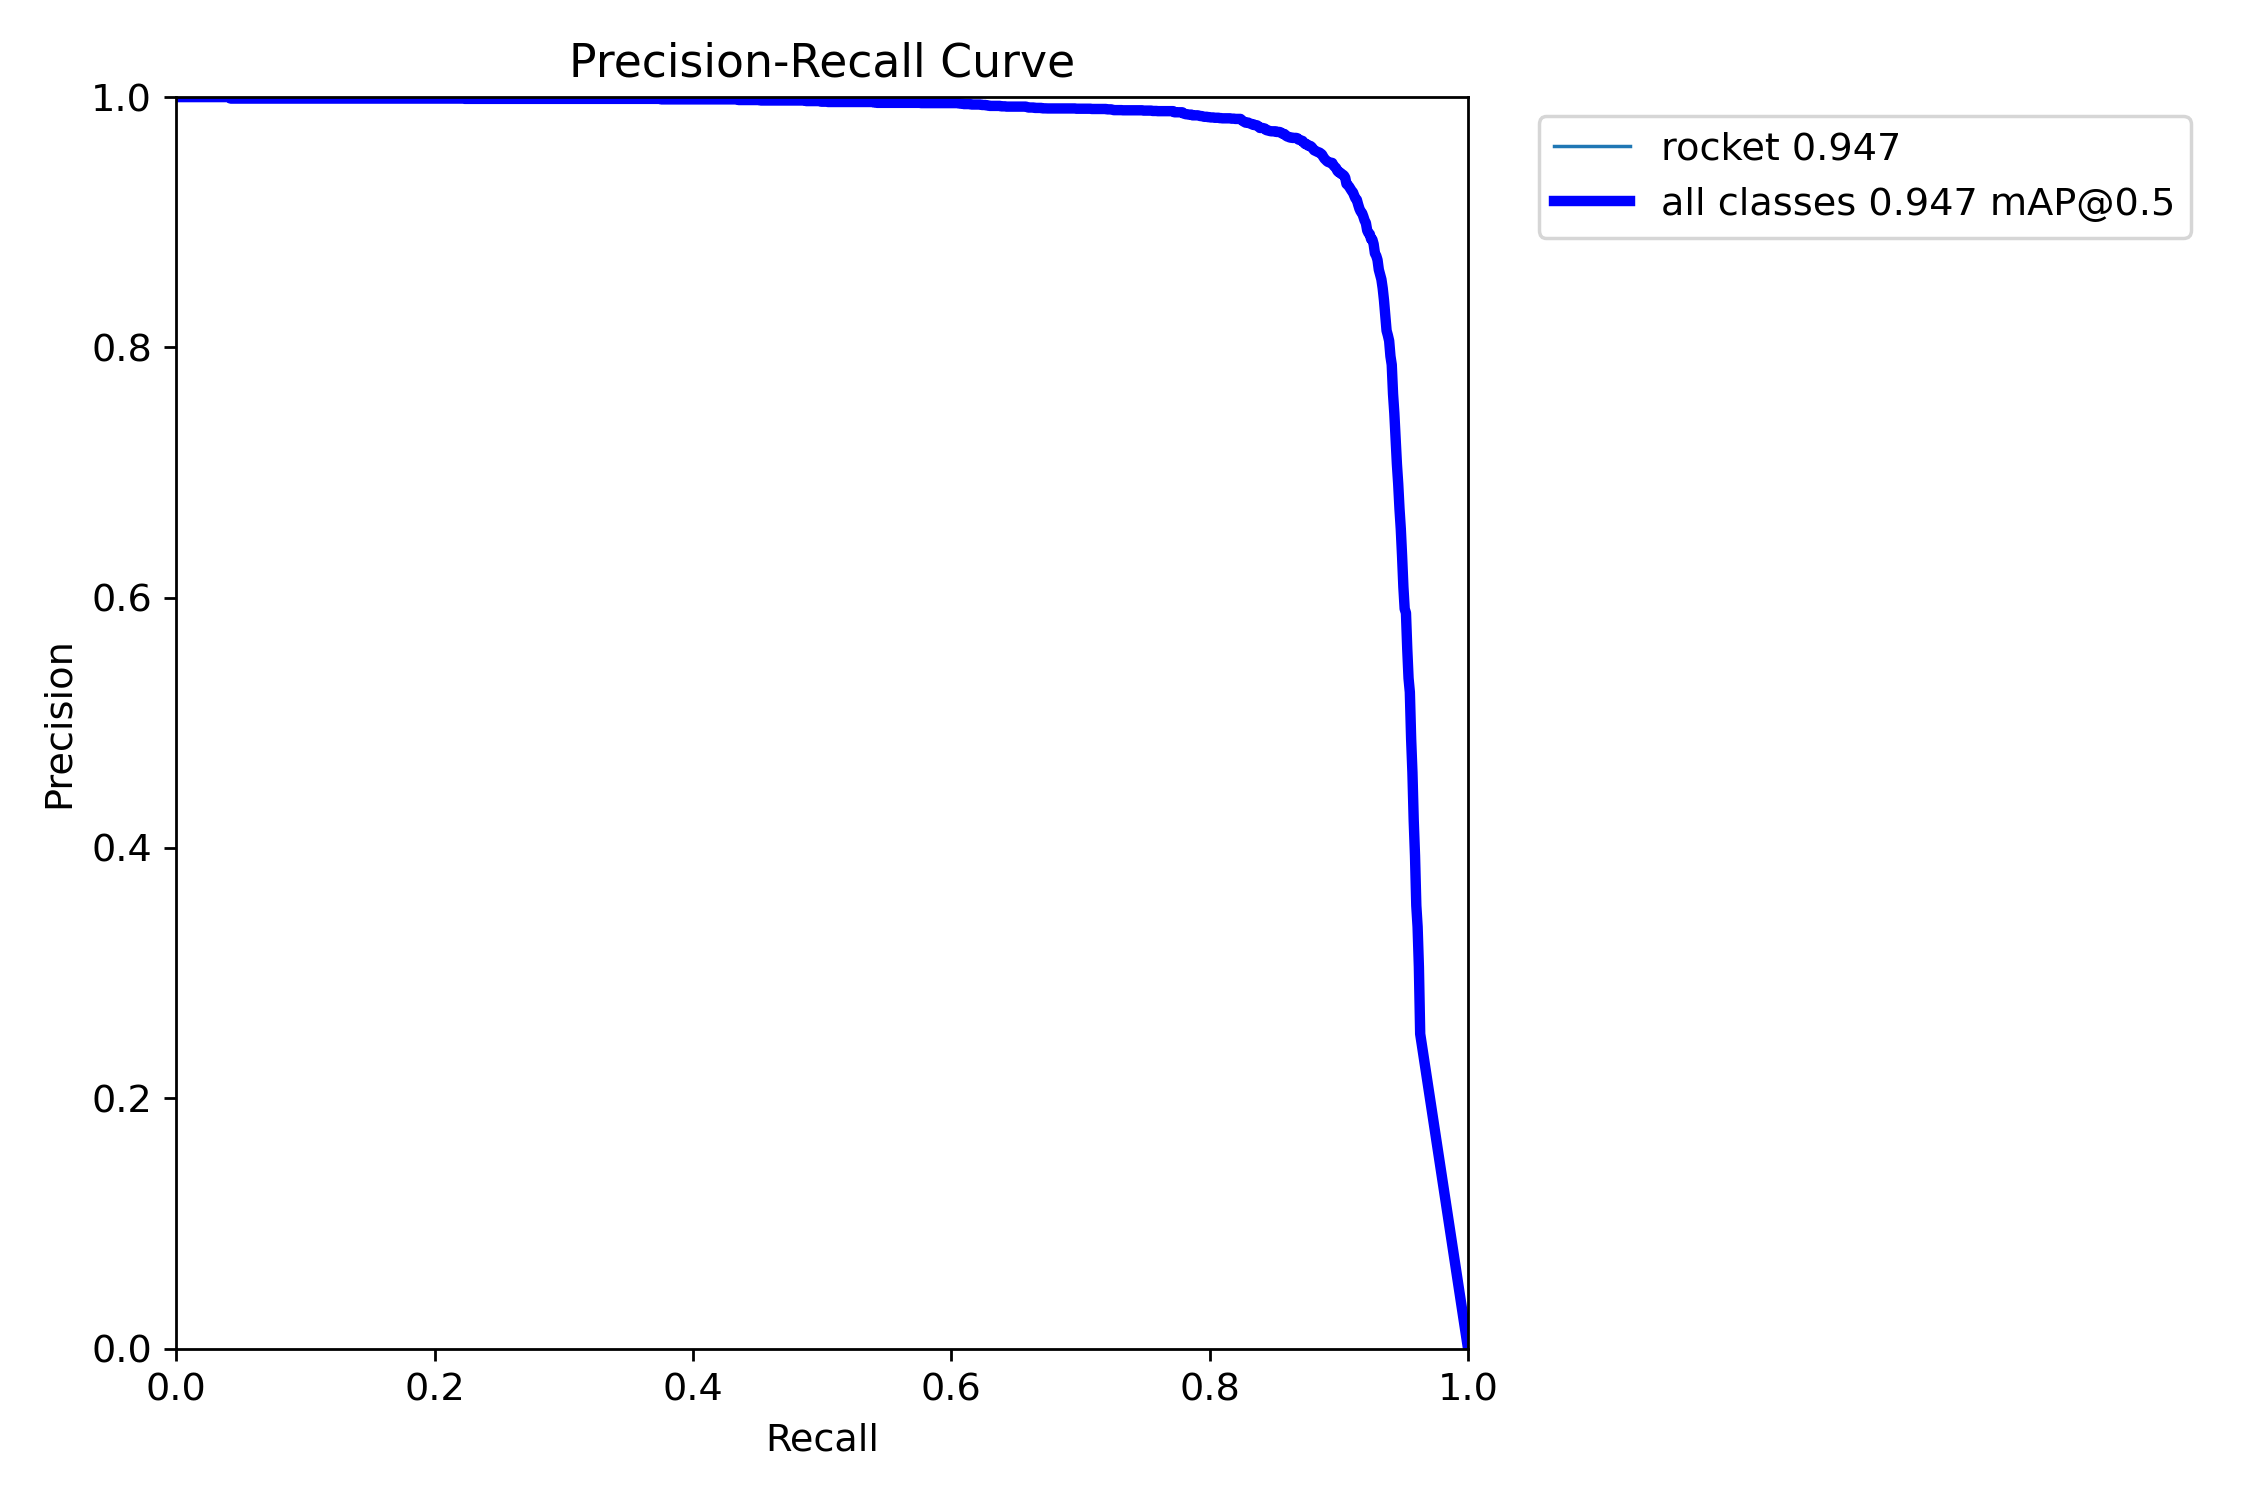
\includegraphics[width=\textwidth]{pr_train63.png}
    \caption{Precision--Recall curve}
  \end{subfigure}
  \hfill
  \begin{subfigure}[t]{0.48\textwidth}
    \centering
    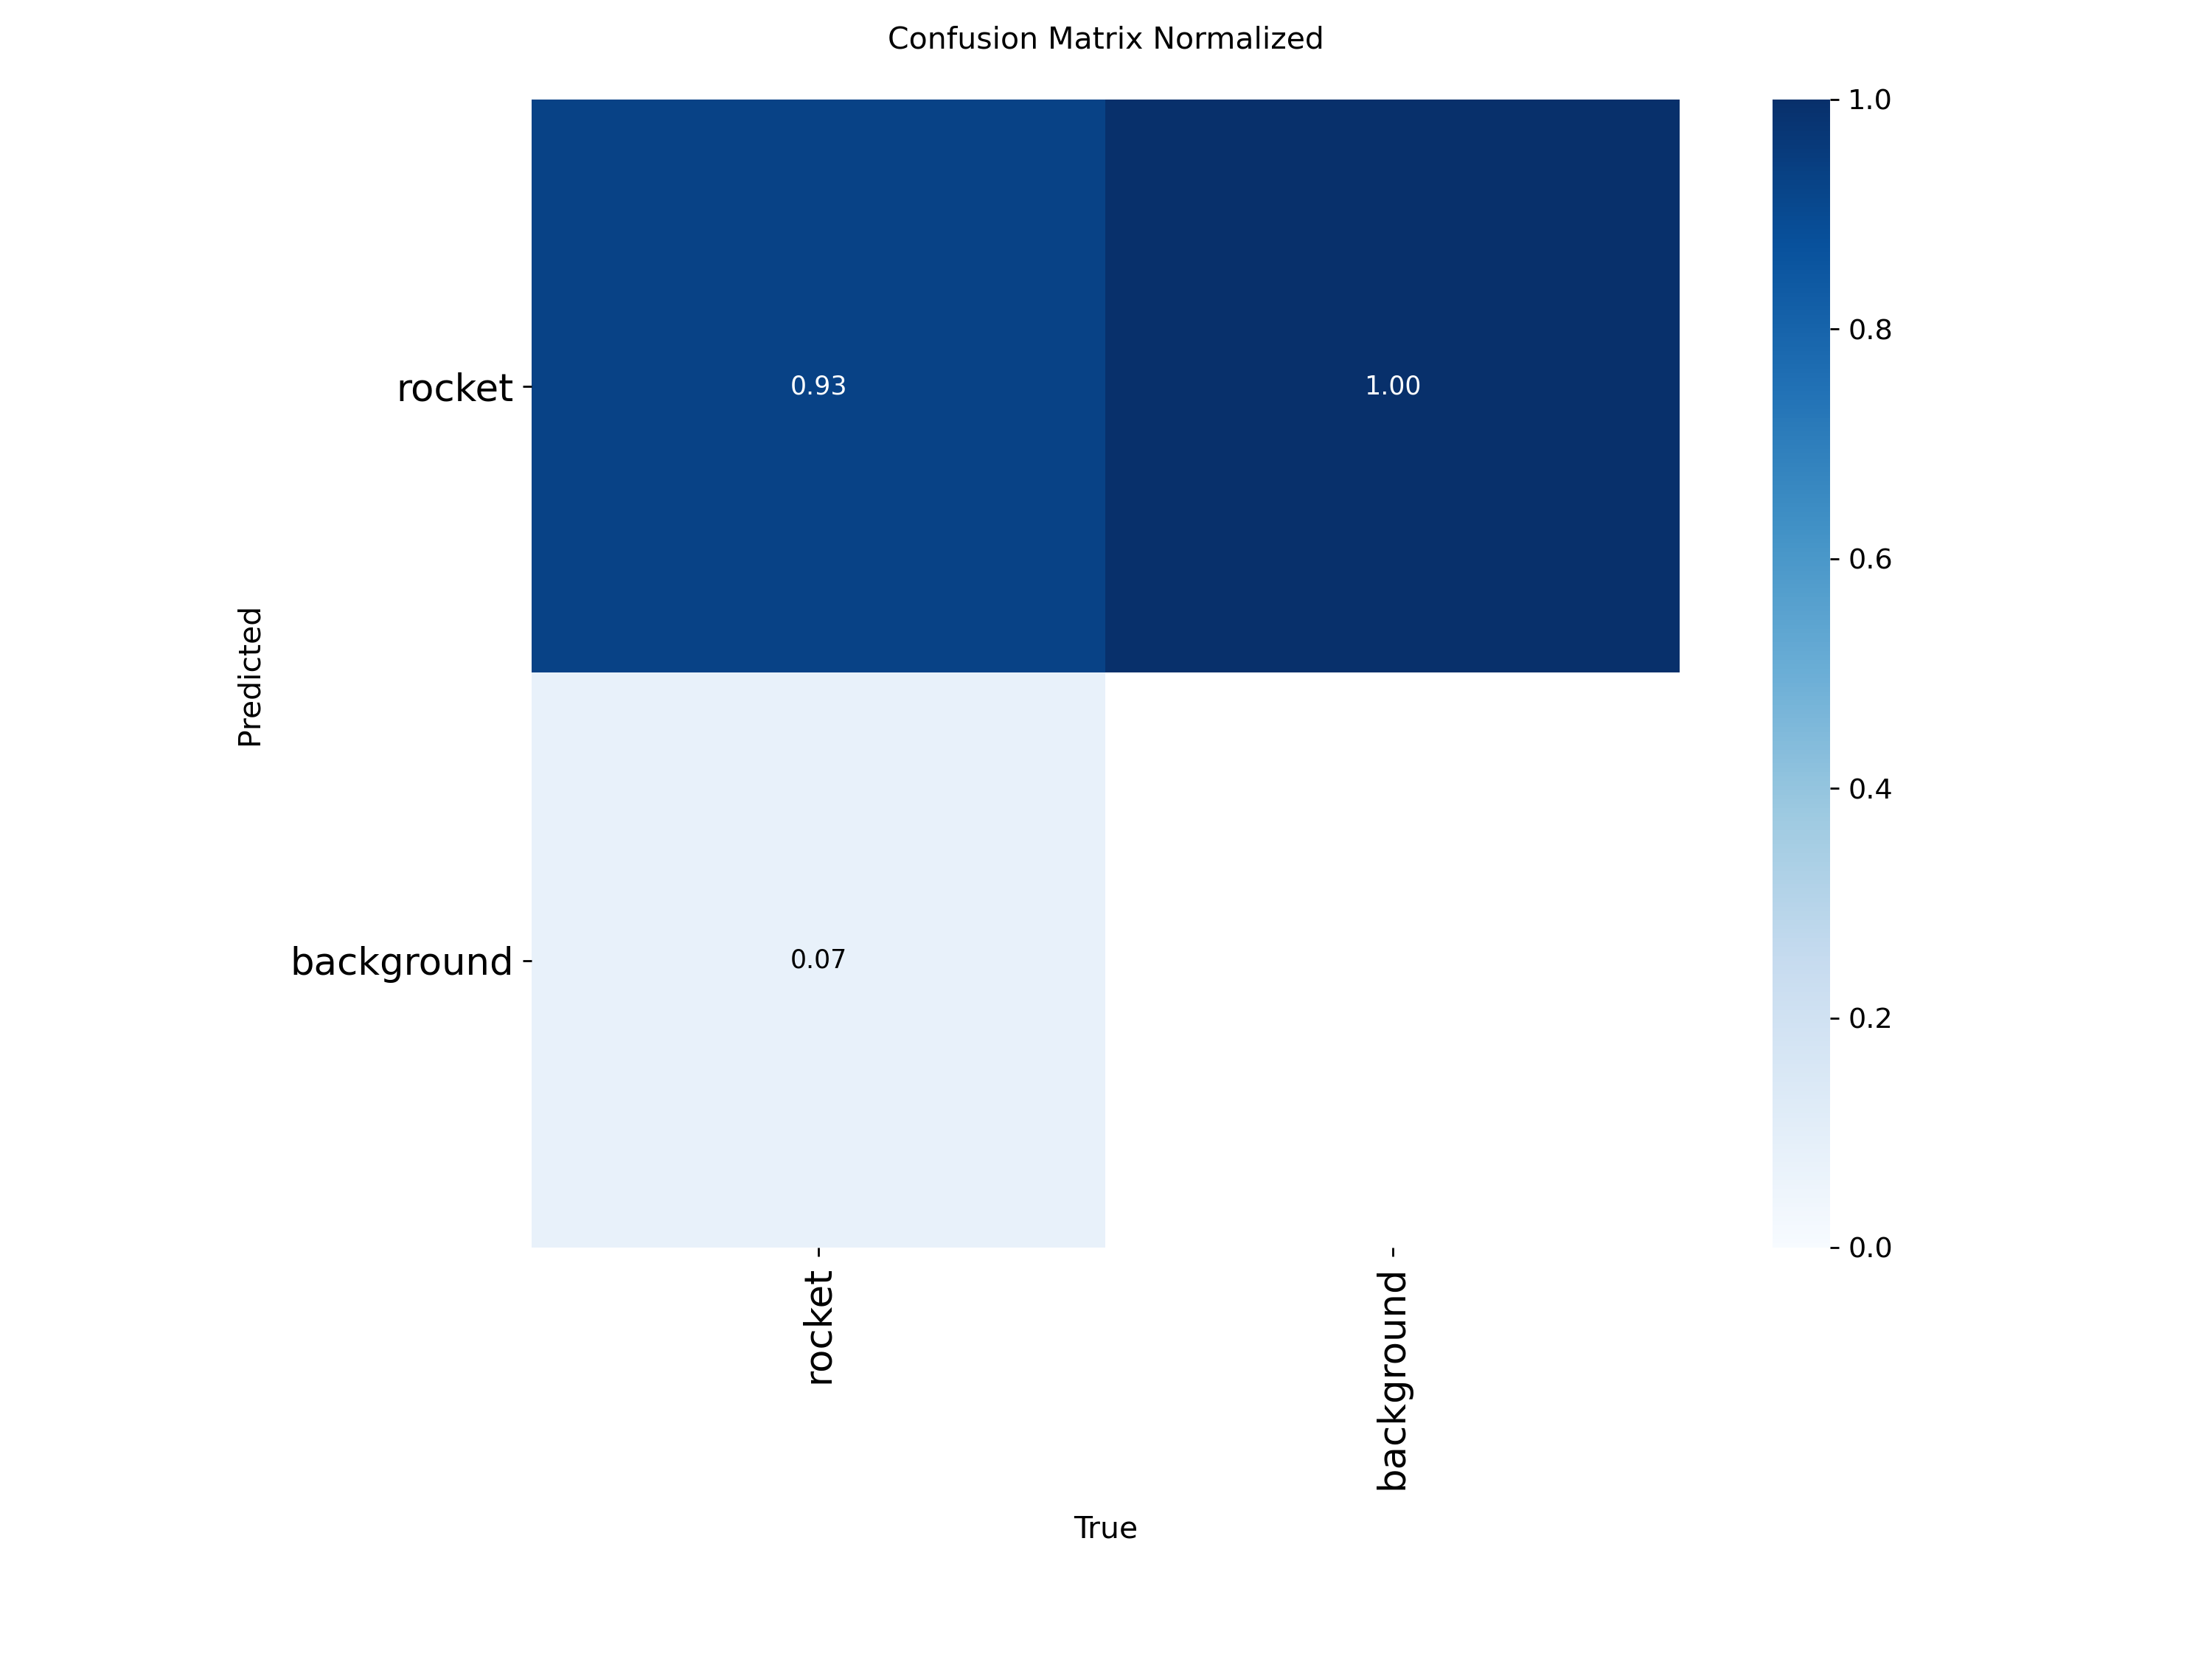
\includegraphics[width=\textwidth]{cm_train63.png}
    \caption{Normalised confusion matrix}
  \end{subfigure}
  \caption{Precision--Recall curve and confusion matrix for the deployed
    model.  The PR curve shows strong performance across all confidence
    thresholds with mAP$_{50} = 0.947$.}
  \label{fig:pr_cm}
\end{figure}

\subsection{Label Distribution and Qualitative Results}

\begin{figure}[H]
  \centering
  \begin{subfigure}[t]{0.48\textwidth}
    \centering
    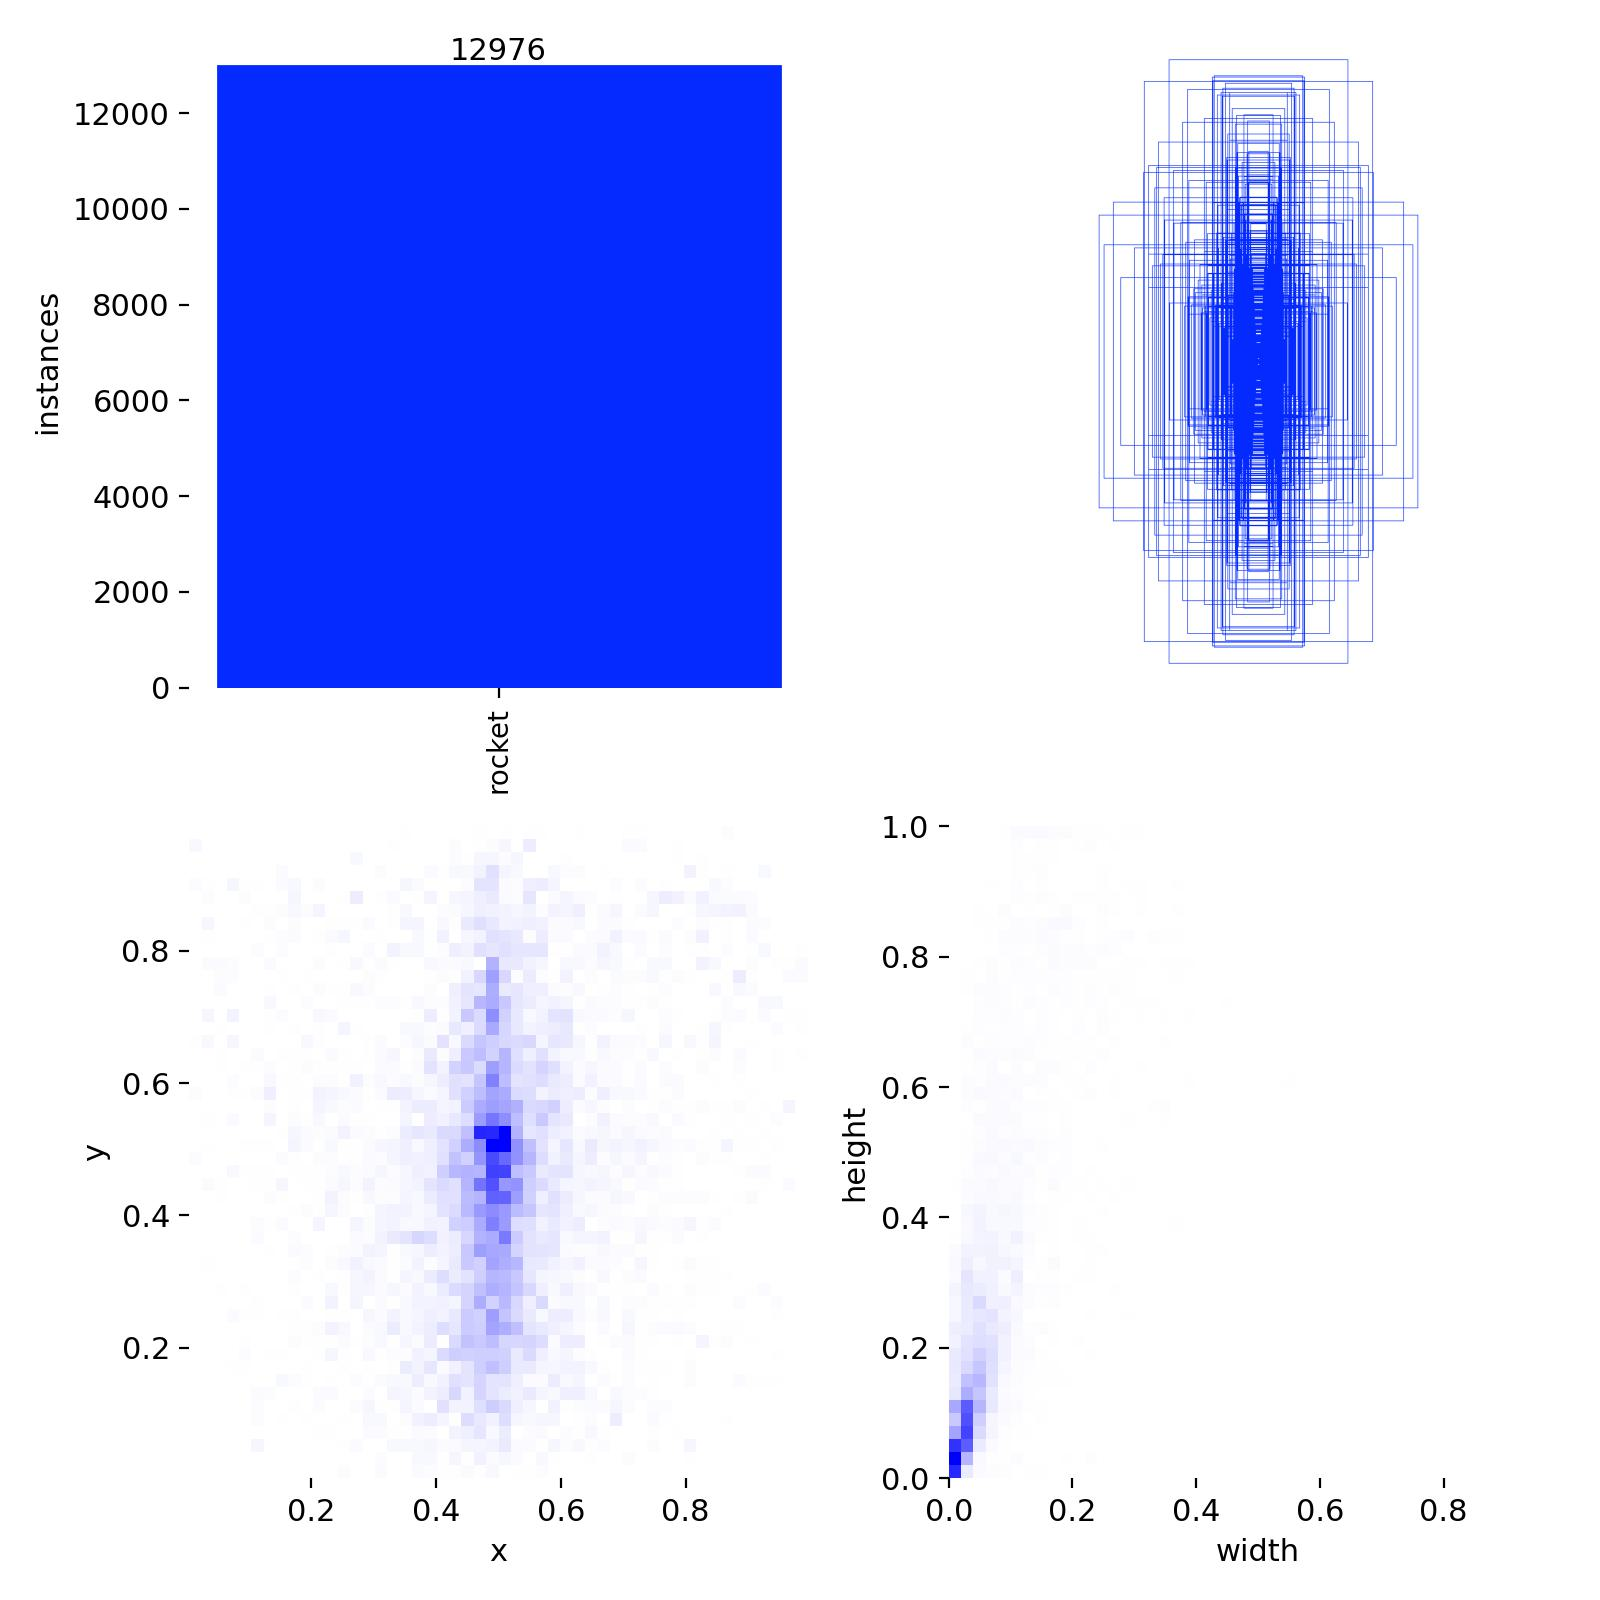
\includegraphics[width=\textwidth]{labels_train63.jpg}
    \caption{Training label distribution}
  \end{subfigure}
  \hfill
  \begin{subfigure}[t]{0.48\textwidth}
    \centering
    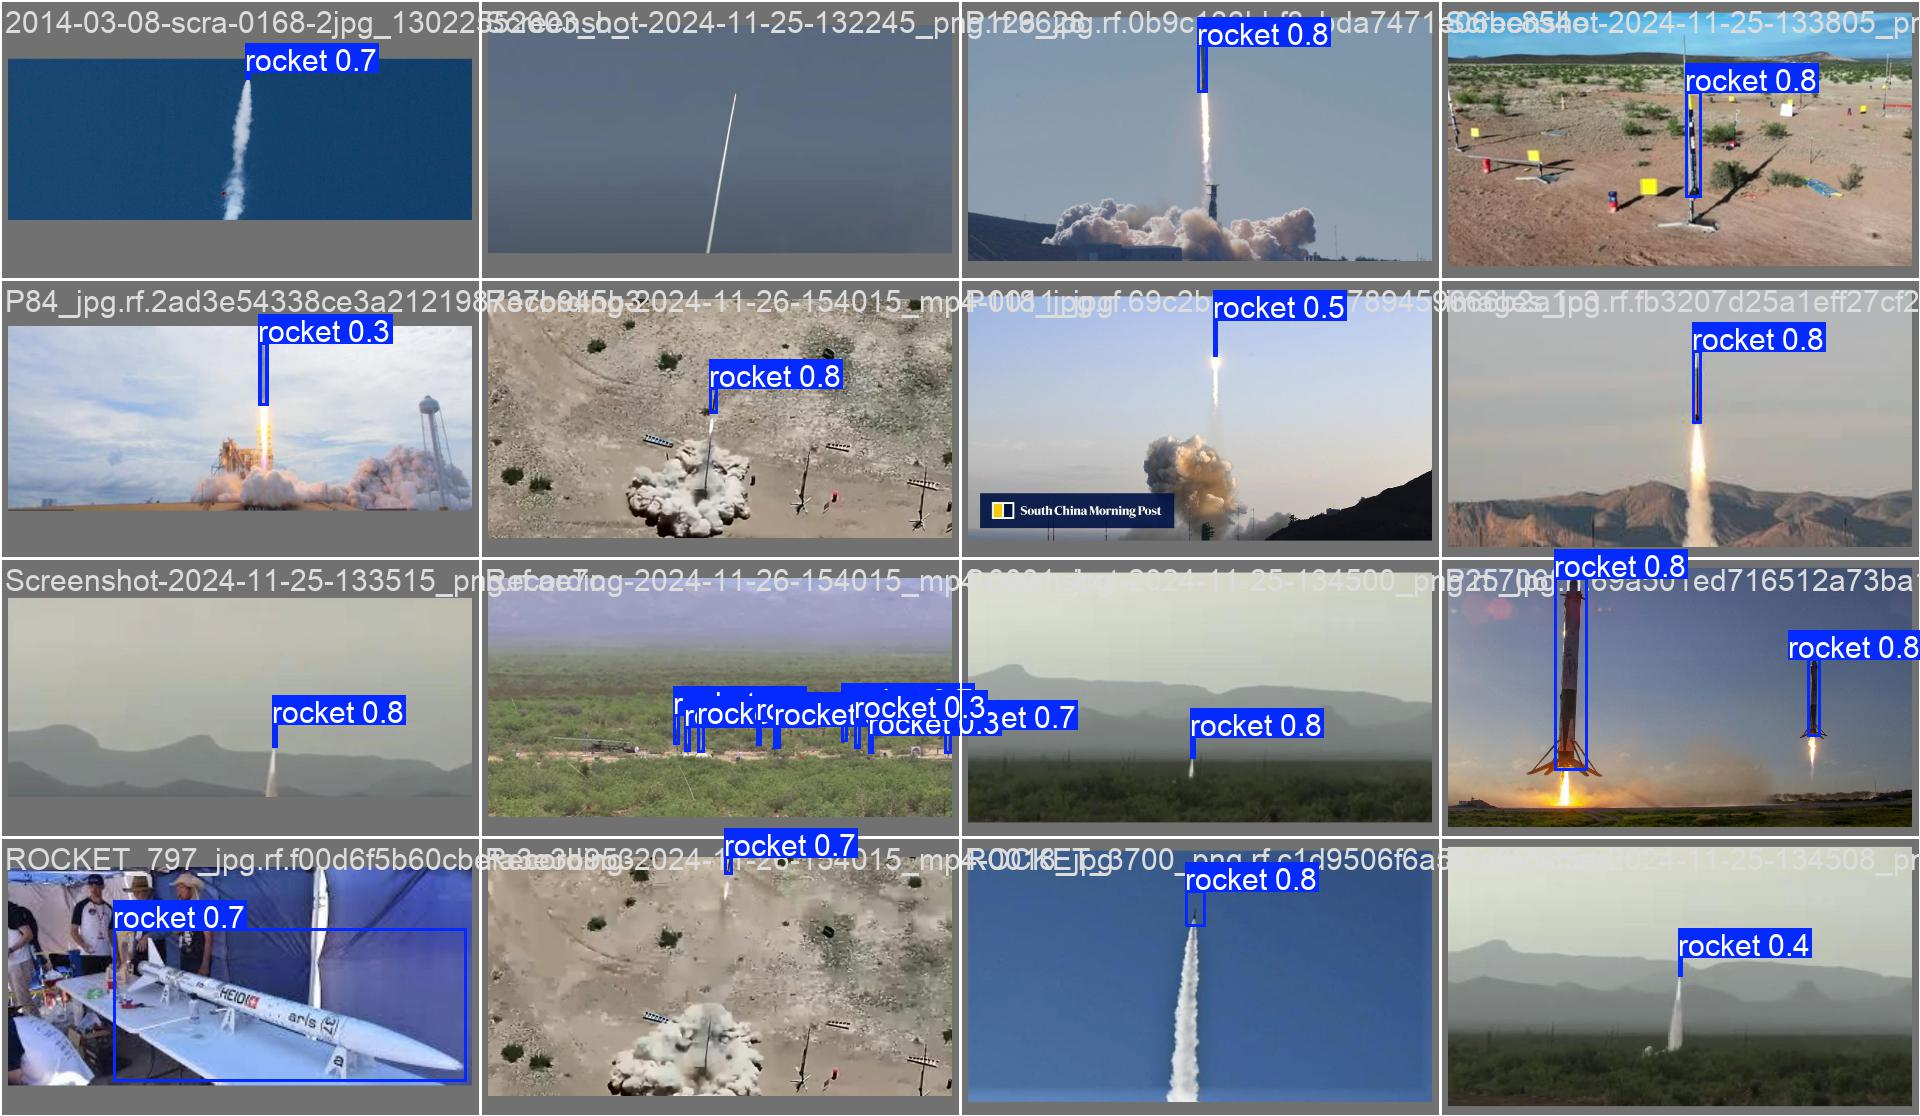
\includegraphics[width=\textwidth]{val_pred_train63.jpg}
    \caption{Validation batch predictions}
  \end{subfigure}
  \caption{(a)~Training label distribution showing the spatial and size
    distribution of rocket annotations.  (b)~Sample validation predictions
    demonstrating accurate detection across various target sizes.}
  \label{fig:labels_qual}
\end{figure}

%% ====================================================================
\section{P2 Architecture Investigation}
\label{sec:p2_failure}
%% ====================================================================

Prior to selecting the standard \textsc{Yolo26s}, we extensively investigated
the \textsc{Yolo26s-P2} variant with a stride-4 detection head, hypothesising
that higher spatial resolution would improve small-object detection.

\subsection{P2 Architecture}

The P2 variant adds a fourth detection head at stride~4, operating on a
feature map with $4{\times}$ the spatial resolution of the standard finest
level (stride~8).

\begin{table}[h]
  \centering
  \caption{Architecture comparison: standard vs.\ P2.}
  \label{tab:arch_compare}
  \begin{tabular}{@{}lccc@{}}
    \toprule
    \textbf{Model}      & \textbf{Parameters} & \textbf{Layers} & \textbf{Detection Strides} \\
    \midrule
    \textsc{Yolo26s}    & 9.47M               & 454             & $\{8, 16, 32\}$            \\
    \textsc{Yolo26s-P2} & 9.66M               & 329             & $\{4, 8, 16, 32\}$         \\
    \bottomrule
  \end{tabular}
\end{table}

\subsection{P2 Training Results}

Through a three-stage fine-tuning protocol (V1) and subsequent regime-consistent
training (V3), the P2 model achieved impressive training metrics:

\begin{table}[H]
  \centering
  \caption{Best P2 training results across pipeline iterations.}
  \label{tab:p2_train}
  \small
  \begin{tabular}{@{}llcccc@{}}
    \toprule
    \textbf{Pipeline} & \textbf{Stage}   & \textbf{P} & \textbf{R} & \textbf{mAP$_{50}$} &
    \textbf{mAP$_{50\text{-}95}$} \\
    \midrule
    V1                & Stage~III        & 0.961      & 0.915      & 0.958               & 0.750 \\
    V2                & Stage~1b         & 0.958      & 0.912      & 0.960               & 0.762 \\
    V3                & Phase~2          & 0.960      & 0.915      & 0.962               & \textbf{0.765} \\
    \bottomrule
  \end{tabular}
\end{table}

\subsection{Deployment Failure}

Despite achieving $\text{mAP}_{50\text{-}95} = 0.765$ in FP32 training
($+10.2\%$ over baseline), the P2 model catastrophically degrades under
FP16 quantisation on the Jetson Orin Nano:

\begin{table}[H]
  \centering
  \caption{Deployment comparison: standard vs.\ P2.}
  \label{tab:p2_deploy}
  \begin{tabular}{@{}lcccc@{}}
    \toprule
    \textbf{Model}    & \textbf{Val mAP} & \textbf{DS mAP} & \textbf{DS small} & \textbf{Quant.\ gap} \\
    \midrule
    \textsc{Yolo26s}  & 0.694            & \textbf{0.631}  & \textbf{0.341}    & $-9.1\%$             \\
    \textsc{Yolo26s-P2} & \textbf{0.765} & 0.539           & 0.150             & $-29.5\%$            \\
    \bottomrule
  \end{tabular}
\end{table}

\paragraph{Key finding.}  The P2 model's training mAP$_{50\text{-}95}$ is
$+10.2\%$ better than the baseline, but its deployment mAP is $-14.6\%$
\emph{worse}.  The quantisation gap is $3.2{\times}$ larger for the P2 model
($-29.5\%$ vs.\ $-9.1\%$).

\subsection{Root Cause: FP16 Quantisation Sensitivity}

The stride-4 detection head operates on feature maps at $240{\times}240$
resolution (for $960{\times}960$ input), producing $16{\times}$ more spatial
positions than the stride-8 head ($120{\times}120$).  FP16's reduced numerical
precision (${\sim}3$ decimal digits vs.\ ${\sim}7$ in FP32) causes:

\begin{enumerate}[leftmargin=*]
  \item \textbf{Spatial precision loss}: Fine-grained positional encoding
        in the stride-4 feature map is quantised away, degrading small-object
        localisation.
  \item \textbf{Activation range compression}: The high-resolution head
        produces activations with a wider dynamic range that FP16 cannot
        faithfully represent.
  \item \textbf{Accumulated rounding}: More layers operating at high
        resolution means more sequential rounding errors.
\end{enumerate}

\paragraph{Lesson.}  Architecture selection for edge deployment must be
validated \textbf{end-to-end at the target precision}.  Training metrics
alone are insufficient---the P2 model's $+10.2\%$ training advantage became
a $-14.6\%$ deployment disadvantage.

%% ====================================================================
\section{Improvement Efforts}
\label{sec:improvements}
%% ====================================================================

Building on the baseline deployed model (DS mAP$_{50\text{-}95} = 0.631$),
we are investigating several strategies to improve small-object detection
while maintaining FP16 deployment compatibility.

\begin{table}[H]
  \centering
  \caption{Ongoing improvement experiments.  Target:
    DS mAP$_{50\text{-}95} > 0.631$ and DS small $> 0.341$.}
  \label{tab:improvements}
  \small
  \begin{tabular}{@{}lp{5.5cm}cc@{}}
    \toprule
    \textbf{Plan} & \textbf{Strategy} & \textbf{Status} & \textbf{DS mAP} \\
    \midrule
    D & Fine-tune smallrocket at 544$\times$960 &
        Complete & 0.641 (small: 0.312) \\
    G & Clone train63 recipe, 150\,ep fine-tune &
        Complete & 0.621 (small: 0.282) \\
    H & From-scratch with enhanced augmentation, 420\,ep &
        Training & --- \\
    I & Tiled (SAHI) training with 50K mixed images &
        Training & --- \\
    J & Copy-paste augmentation, 420\,ep &
        Training & --- \\
    \bottomrule
  \end{tabular}
\end{table}

Plans~D and G confirm that fine-tuning from the baseline tends to
\emph{improve} overall mAP but \emph{regress} small-object detection.
Plans~H, I, and J explore from-scratch training with augmentation strategies
specifically targeting small objects.

%% ====================================================================
\section{Conclusion}
\label{sec:conclusion}
%% ====================================================================

We have presented the training methodology and deployment pipeline for a
small-rocket detection system achieving
DS~mAP$_{50\text{-}95} = \mathbf{0.631}$ and
DS~mAP$_{50\text{-}95}(\text{small}) = \mathbf{0.341}$ on the Jetson Orin
Nano with TensorRT FP16.  The key insights are:

\begin{enumerate}[leftmargin=*]
  \item \textbf{Full mosaic is non-negotiable for small objects.}  Setting
        $\text{mosaic} = 1.0$ with $\texttt{close\_mosaic} = 80$ provides
        the best balance of augmented feature diversity and full-resolution
        refinement.  All reduced-mosaic variants underperformed.

  \item \textbf{Deployment metrics must drive model selection.}  The P2
        architecture achieves $+10.2\%$ higher training mAP but $-14.6\%$
        lower deployment mAP due to FP16 quantisation sensitivity.
        Training-only evaluation would have led to the wrong model choice.

  \item \textbf{COCO hard negatives suppress false positives.}  Injecting
        4{,}000 pure background images (25\% of training set) forces a harder
        decision boundary, which is critical for real-world deployment.

  \item \textbf{Multi-scale training improves robustness.}  Variable input
        resolution ($544$--$960$\,px) with $\texttt{multi\_scale}=\text{True}$
        produces scale-invariant features essential for the extreme size range
        in our dataset.

  \item \textbf{Custom Albumentations target deployment conditions.}  Seven
        transforms targeting motion blur, sensor noise, compression artefacts,
        and illumination variation improve robustness to real-world imaging
        degradation.

  \item \textbf{The quantisation gap is architecture-dependent.}  Standard
        \textsc{Yolo26s} loses $9.1\%$ under FP16, while \textsc{Yolo26s-P2}
        loses $29.5\%$---architectures with high-resolution feature maps are
        disproportionately affected.
\end{enumerate}

\noindent Ongoing experiments (Plans~H, I, J) explore from-scratch training
with enhanced augmentation, tiled (SAHI) training, and copy-paste augmentation
to improve small-object detection beyond the current baseline.

\bibliographystyle{plainnat}

\bibliography{../../../refs/References}

\newpage

\appendix

%% ====================================================================
\section{Hardware Configuration}
\label{app:hardware}
%% ====================================================================

\begin{table}[H]
  \centering
  \caption{Training and deployment infrastructure.}
  \label{tab:hardware}
  \begin{tabular}{@{}lll@{}}
    \toprule
    \textbf{Component}  & \textbf{Training (Grace HPC)}          & \textbf{Deployment (Orin)}      \\
    \midrule
    Device              & NVIDIA H100 PCIe, 80\,GB               & NVIDIA Jetson Orin Nano, 8\,GB  \\
    Training mode       & Single GPU                             & ---                             \\
    Precision           & AMP (FP16/FP32)                        & TensorRT FP16                   \\
    Framework           & Ultralytics (PyTorch)                  & DeepStream + TensorRT           \\
    Disk cache          & Enabled                                & ---                             \\
    \midrule
    Server              & McMaster Grace HPC, RHEL 9             & Jetson Orin Nano (on-site)      \\
    \bottomrule
  \end{tabular}
\end{table}

%% ====================================================================
\section{Complete Training Hyperparameters}
\label{app:hyperparams}
%% ====================================================================

\begin{table}[H]
  \centering
  \caption{Full \texttt{args.yaml} for train63 (deployed model).}
  \label{tab:full_hyper}
  \footnotesize
  \begin{tabular}{@{}llll@{}}
    \toprule
    \textbf{Category}   & \textbf{Parameter}   & \textbf{Value}   & \textbf{Notes}        \\
    \midrule
    \multirow{8}{*}{Core}
                         & model                & yolo26s.pt       & COCO pretrained       \\
                         & data                 & data\_15000      & 15{,}832 train images \\
                         & imgsz                & (544, 960)       & Rectangular           \\
                         & batch                & 64               &                       \\
                         & epochs               & 420              & Full training         \\
                         & device               & 0                & Single H100           \\
                         & amp                  & True             &                       \\
                         & multi\_scale         & True             & 544--960\,px range    \\
    \midrule
    \multirow{6}{*}{Optimiser}
                         & optimizer            & auto (SGD)       &                       \\
                         & lr0                  & 0.01             &                       \\
                         & lrf                  & 0.01             & Linear decay          \\
                         & cos\_lr              & False            &                       \\
                         & momentum             & 0.937            &                       \\
                         & weight\_decay        & 0.0005           &                       \\
    \midrule
    \multirow{6}{*}{Augmentation}
                         & mosaic               & 1.0              & Always on             \\
                         & close\_mosaic        & 80               & Off last 80\,ep       \\
                         & mixup                & 0.1              &                       \\
                         & cutmix               & 0.1              &                       \\
                         & copy\_paste          & 0.0              &                       \\
                         & erasing              & 0.4              &                       \\
    \midrule
    \multirow{6}{*}{Geometric}
                         & degrees              & 180              & Full rotation         \\
                         & flipud               & 0.5              &                       \\
                         & fliplr               & 0.5              &                       \\
                         & shear                & 5.0              &                       \\
                         & perspective          & 0.0002           &                       \\
                         & scale                & 0.3              &                       \\
    \midrule
    \multirow{3}{*}{Colour}
                         & hsv\_h               & 0.015            &                       \\
                         & hsv\_s               & 0.6              &                       \\
                         & hsv\_v               & 0.4              &                       \\
    \midrule
    \multirow{3}{*}{Control}
                         & patience             & 30               &                       \\
                         & save\_period          & 25               &                       \\
                         & seed                 & 0                &                       \\
    \bottomrule
  \end{tabular}
\end{table}

%% ====================================================================
\section{P2 Training History}
\label{app:p2_history}
%% ====================================================================

For completeness, Table~\ref{tab:p2_history} documents the full P2 training
progression across three pipeline iterations.

\begin{table}[H]
  \centering
  \caption{P2 training history across V1/V2/V3 pipelines.  Despite reaching
    mAP$_{50\text{-}95} = 0.765$, the model was not deployed due to FP16
    quantisation failure.}
  \label{tab:p2_history}
  \small
  \begin{tabular}{@{}lllccc@{}}
    \toprule
    \textbf{Pipeline} & \textbf{Stage}   & \textbf{Strategy}         &
    \textbf{Epochs}   & \textbf{Best Ep.} & \textbf{mAP$_{50\text{-}95}$} \\
    \midrule
    V1 & Stage~I   & P2 + COCO neg, 4-GPU DDP          & 600  & 267 & 0.614 \\
    V1 & Stage~II  & Close-mosaic fine-tune             & 100  & 93  & 0.720 \\
    V1 & Stage~III & Ultra-fine polish, SGD             & 60   & 52  & 0.750 \\
    V2 & Stage~1b  & Extended DDP, SGD throughout       & 300  & 283 & 0.762 \\
    V3 & Phase~1   & Regime-consistent, native aug      & 250  & 233 & 0.754 \\
    V3 & Phase~2   & Low-LR fine-tune                   & 80   & 37  & \textbf{0.765} \\
    \bottomrule
  \end{tabular}
\end{table}

\end{document}
